\documentclass[12pt,a4paper]{article}

% --- PACKAGES ---
\usepackage[utf8]{inputenc}
\usepackage[T1]{fontenc}      % Font encoding
\usepackage{amsmath}
\usepackage{amsfonts}         % Math fonts package
\usepackage{amssymb}          % Math symbols package
\usepackage{graphicx}         % Required for including images
\usepackage[a4paper, margin=1in]{geometry} % For page margins
\usepackage{times}            % Uses Times New Roman like font
\usepackage{setspace}         % For line spacing
\usepackage{hyperref}         % For clickable links

\usepackage{fancyhdr}         % For custom headers and footers
\usepackage{caption}          % For customizing captions
% \usepackage{subcaption}       % For subfigures (if needed)
% \usepackage{float}            % For better figure placement with [H] (if needed)
% \usepackage{tikz}             % For diagrams (if needed)
% \usetikzlibrary{shapes.geometric, arrows, positioning, fit} % TikZ libraries (if needed)

\usepackage{xcolor}
\usepackage{sectsty}          % To style section headings
\usepackage{tocloft}          % To style Table of Contents
\usepackage{listings}         % For code listings

% --- COLOR DEFINITIONS ---
\definecolor{RoyalBlue}{RGB}{0, 0, 128} % As per your example
\definecolor{codegreen}{rgb}{0,0.6,0}
\definecolor{codegray}{rgb}{0.5,0.5,0.5}
\definecolor{codepurple}{rgb}{0.58,0,0.82}
\definecolor{backcolour}{rgb}{0.95,0.95,0.92}

% --- HYPERREF SETUP ---
\hypersetup{
    colorlinks=true,
    linkcolor=RoyalBlue,
    filecolor=magenta,      
    urlcolor=cyan, % Kept cyan for URLs, you can change to RoyalBlue if preferred
    pdftitle={Retro Pong Challenge: A Python-Based Arcade Game with Unit Testing},
    pdfpagemode=FullScreen,
}

% --- FONT & SECTION STYLING ---
\sectionfont{\color{RoyalBlue}}   % Section titles in document
\subsectionfont{\color{RoyalBlue}} % Subsection titles
\subsubsectionfont{\color{RoyalBlue}}% Subsubsection titles

% --- TABLE OF CONTENTS STYLING ---
\renewcommand{\cfttoctitlefont}{\color{black}\Huge\bfseries} % Title "Contents" in black
\renewcommand{\cftsecfont}{\color{RoyalBlue}}                % Section entries in ToC
\renewcommand{\cftsecpagefont}{\color{RoyalBlue}}            % Section page numbers
\renewcommand{\cftsubsecfont}{\color{RoyalBlue}}              % Subsection entries
\renewcommand{\cftsubsecpagefont}{\color{RoyalBlue}}          % Subsection page numbers
\renewcommand{\cftsubsubsecfont}{\color{RoyalBlue}}           % Subsubsection entries
\renewcommand{\cftsubsubsecpagefont}{\color{RoyalBlue}}       % Subsubsection page numbers

% --- LISTINGS (CODE) SETUP ---
\lstdefinestyle{mystyle}{
    backgroundcolor=\color{backcolour},   
    commentstyle=\color{codegreen},
    keywordstyle=\color{magenta},
    numberstyle=\tiny\color{codegray},
    stringstyle=\color{codepurple},
    basicstyle=\ttfamily\footnotesize,
    breakatwhitespace=false,         
    breaklines=true,                 
    captionpos=b,                    
    keepspaces=true,                 
    numbers=left,                    
    numbersep=5pt,                  
    showspaces=false,                
    showstringspaces=false,
    showtabs=false,                  
    tabsize=2,
    frame=single,
    rulecolor=\color{black}, % Frame color for listings
    title=\lstname % To show the filename if provided in caption
}
\lstset{style=mystyle}

% --- PAGE STYLE FOR CONTENT PAGES ---
\pagestyle{fancy}
\fancyhf{} % Clear all header and footer fields
\fancyhead[C]{\textit{Retro Pong Challenge: Python Game with Unit Testing}} % Custom header
\fancyfoot[C]{\thepage}
\renewcommand{\headrulewidth}{0.4pt}
\renewcommand{\footrulewidth}{0pt} % No footer rule

% --- CUSTOM TITLE PAGE COMMAND ---
\newcommand{\maketitlepage}{
    \begin{titlepage}
        \centering
        \vspace*{0.5cm}
        % 
\includegraphics[width=0.25\textwidth]{RUET_logo.png} % Placeholder for University Logo
        {\Huge \textbf{RAJSHAHI UNIVERSITY OF ENGINEERING \& TECHNOLOGY}}
        \vspace*{0.5cm}
        {\Large Department of Computer Science and Engineering}
        
        \vspace*{2.5cm}
        
        {\huge\bfseries Retro Pong Challenge: A Python-Based Arcade Game with Unit Testing\par}
        \vspace{0.5cm}
        {\Large \textit{A Software Engineering Sessional Project Report}\par} % Subtitle
        
        \vspace{2cm}
        
        \begin{flushleft}
        \large \textbf{Submitted by:}\\
        \large Md Naim Parvez \\
        \large Roll No: 2003015 \\
        \large Section: A \\
        \large Third Year (Even Semester) \\ % Assuming, adjust if needed
        \end{flushleft}
        
        \vspace{1cm}
        
        \begin{flushleft}
        \large \textbf{Submitted to:}\\
        \large Emrana Kabir Hashi \\
        \large Assistant Professor \\
        \large Department of Computer Science and Engineering \\
        \large Rajshahi University of Engineering \& Technology (RUET) \\
        \end{flushleft}
        
        \vspace{1cm}
        {\large \textbf{Course Code:} CSE 3206} \\
        {\large \textbf{Course Title:} Software Engineering Sessional}
        
        \vfill 
        
        {\large April 2025\par} % Submission Date (Matches previous content)
    \end{titlepage}
}

\begin{document}

% --- TITLE PAGE ---
\maketitlepage
\thispagestyle{empty} % No header/footer on the title page

% --- TABLE OF CONTENTS ---
\newpage
\pagenumbering{roman} % Roman numerals for ToC, Abstract etc.
\tableofcontents
\newpage
\pagenumbering{arabic} % Arabic numerals for main content
\setcounter{page}{1} % Start main content page numbering from 1

% --- ABSTRACT ---
\section*{Abstract} % Unnumbered section
\addcontentsline{toc}{section}{Abstract} % Manually add to ToC

Retro Pong Challenge is a Python-based arcade game developed as a university project at Rajshahi University of Engineering \& Technology (RUET). Built using Tkinter for the GUI, the game recreates the classic Pong experience, offering a simple yet engaging interface with distinct paddles and a dynamic ball. Key features include two-player control, real-time score tracking, and a game reset mechanism. The project incorporates comprehensive unit testing using Python's \texttt{unittest} framework with 9 distinct test cases to verify the core game logic, including ball movement, collision detection, and scoring, ensuring robust functionality. This report details the development process, including system design, a conceptual overview of the source code implementation, the comprehensive testing methodology, and anticipated results. The conceptual source code is available on GitHub at \url{https://github.com/Rohan-Ahmed-Student/RetroPongChallenge}. The report also discusses the project's outcomes and potential for future enhancements, such as adding an AI opponent and advanced gameplay modes.

% --- INTRODUCTION ---
\section{Introduction}
\subsection{About the Project}
Retro Pong Challenge is a desktop arcade game developed to provide an entertaining and nostalgic gaming experience. Initiated in 2025, the project utilizes Python's Tkinter library to create a straightforward and responsive interface. It features two-player gameplay where each player controls a paddle, score tracking, and the ability to restart the game. The game involves a ball moving across the screen, bouncing off walls and paddles, with players attempting to hit the ball past their opponent's paddle to score points.

\subsection{Objectives}
The primary objectives of Retro Pong Challenge are:
\begin{itemize}
    \item To develop an interactive Pong game with a clean, retro-inspired UI.
    \item To implement keyboard-based controls for two players to maneuver their respective paddles.
    \item To accurately track scores and declare a winner when a predefined score is reached.
    \item To provide options to reset the game for a new match.
    \item To apply comprehensive unit testing to verify the core game logic, including ball physics, collision detection, and scoring mechanisms.
    \item To ensure the code is well-structured, maintainable, and allows for future enhancements.
    \item To demonstrate software testing principles and best practices in a practical application.
\end{itemize}

\subsection{System Requirement Analysis}
The system requirements were formulated based on the classic Pong game mechanics and discussions regarding project scope. The requirements include:
\begin{itemize}
    \item \textbf{Functional Requirements:}
    \begin{itemize}
        \item Independent vertical movement of two paddles via keyboard input.
        \item Continuous ball movement with realistic bounces off top/bottom walls and paddles.
        \item Accurate scoring when the ball passes an opponent's paddle.
        \item Declaration of a winner upon reaching 7 points.
        \item Game reset functionality to start a new match with scores at zero.
        \item Comprehensive unit tests covering all core game logic methods.
    \end{itemize}
    \item \textbf{Non-Functional Requirements:}
    \begin{itemize}
        \item Responsive and clear UI with a retro arcade aesthetic (e.g., black background, white/colored elements).
        \item Maintainable and modular code structure.
        \item 100\% test coverage for game logic methods.
    \end{itemize}
    \item \textbf{Hardware Requirements:}
    \begin{itemize}
        \item A computer with at least 2GB RAM and a 1GHz processor.
    \end{itemize}
    \item \textbf{Software Requirements:}
    \begin{itemize}
        \item Python 3.10+ with Tkinter support.
        \item \texttt{unittest} framework for testing.
        \item A development environment such as Visual Studio Code.
    \end{itemize}
\end{itemize}

% --- SYSTEM DESIGN AND DEVELOPMENT ---
\section{System Design and Development}
\subsection{Architecture Overview}
The system is designed with a modular architecture, separating game logic from the user interface:
\begin{itemize}
    \item \textbf{\texttt{PongGameLogic} Class:} Encapsulates all game logic, including managing ball position and velocity, paddle positions, collision detection with walls and paddles, score updates, and game state (e.g., determining a winner).
    \item \textbf{\texttt{PongGameGUI} Class:} Manages the GUI components using Tkinter, handles user input (keyboard events for paddle movement), and orchestrates the visual representation of the game, including drawing paddles, the ball, and the scoreboard.
    \item \textbf{Test Suite:} A comprehensive set of unit tests to validate the functionality of the \texttt{PongGameLogic} class.
\end{itemize}

\subsection{Complete Source Code Implementation (Conceptual)}
This section provides a conceptual outline of the main game implementation.

\subsubsection{Main Game Implementation (\texttt{pong\_game.py})}
\begin{lstlisting}[language=Python, caption={Conceptual \texttt{pong\_game.py} Implementation}, label={lst:pong_game}]
# Conceptual Outline for pong_game.py
import tkinter as tk
import time # Not strictly used in this conceptual GUI logic but common

# --- Constants ---
SCREEN_WIDTH = 800
SCREEN_HEIGHT = 600
PADDLE_WIDTH = 20
PADDLE_HEIGHT = 100
BALL_RADIUS = 10
PADDLE_SPEED = 30 # Speed of paddle movement
BALL_SPEED_X_INITIAL = 5 # Initial X-speed of ball
BALL_SPEED_Y_INITIAL = 5 # Initial Y-speed of ball
WINNING_SCORE = 7

# Colors
BG_COLOR = '#000000'       # Black
PADDLE_COLOR = '#FFFFFF'   # White
BALL_COLOR = '#FFFF00'     # Yellow
TEXT_COLOR = '#FFFFFF'     # White

# --- Game Logic Class ---
class PongGameLogic:
    def __init__(self):
        self.ball_pos = [SCREEN_WIDTH / 2, SCREEN_HEIGHT / 2]
        self.ball_vel = [BALL_SPEED_X_INITIAL, BALL_SPEED_Y_INITIAL]
        self.paddle1_pos_y = SCREEN_HEIGHT / 2 - PADDLE_HEIGHT / 2
        self.paddle2_pos_y = SCREEN_HEIGHT / 2 - PADDLE_HEIGHT / 2
        self.score1 = 0
        self.score2 = 0
        self.game_over_flag = False

    def update_ball(self):
        if self.game_over_flag:
            return

        self.ball_pos[0] += self.ball_vel[0]
        self.ball_pos[1] += self.ball_vel[1]

        # Wall collision (top/bottom)
        if self.ball_pos[1] - BALL_RADIUS <= 0 or \
           self.ball_pos[1] + BALL_RADIUS >= SCREEN_HEIGHT:
            self.ball_vel[1] *= -1

        # Paddle collision
        # Paddle 1 (left)
        if self.ball_pos[0] - BALL_RADIUS <= PADDLE_WIDTH and \
           self.paddle1_pos_y < self.ball_pos[1] < self.paddle1_pos_y + PADDLE_HEIGHT:
            if self.ball_vel[0] < 0: # Check if ball is moving towards paddle
                self.ball_vel[0] *= -1
        
        # Paddle 2 (right)
        if self.ball_pos[0] + BALL_RADIUS >= SCREEN_WIDTH - PADDLE_WIDTH and \
           self.paddle2_pos_y < self.ball_pos[1] < self.paddle2_pos_y + PADDLE_HEIGHT:
            if self.ball_vel[0] > 0: # Check if ball is moving towards paddle
                self.ball_vel[0] *= -1

        # Scoring
        if self.ball_pos[0] - BALL_RADIUS < 0: # Ball passed paddle 1 (left edge)
            self.score2 += 1
            self.reset_ball()
        elif self.ball_pos[0] + BALL_RADIUS > SCREEN_WIDTH: # Ball passed paddle 2 (right edge)
            self.score1 += 1
            self.reset_ball()
        
        self.check_game_over()

    def reset_ball(self):
        self.ball_pos = [SCREEN_WIDTH / 2, SCREEN_HEIGHT / 2]
        # Alternate starting direction for fairness
        self.ball_vel[0] *= -1 
        # Optionally randomize Y velocity or keep it consistent

    def move_paddle(self, paddle_num, direction): # direction: -1 for up, 1 for down
        if paddle_num == 1:
            self.paddle1_pos_y += PADDLE_SPEED * direction
            # Boundary checks for paddle 1
            self.paddle1_pos_y = max(0, min(self.paddle1_pos_y, SCREEN_HEIGHT - PADDLE_HEIGHT))
        elif paddle_num == 2:
            self.paddle2_pos_y += PADDLE_SPEED * direction
            # Boundary checks for paddle 2
            self.paddle2_pos_y = max(0, min(self.paddle2_pos_y, SCREEN_HEIGHT - PADDLE_HEIGHT))

    def check_game_over(self):
        if self.score1 >= WINNING_SCORE or self.score2 >= WINNING_SCORE:
            self.game_over_flag = True
            return True
        return False

    def reset_game_state(self): # For full game reset (e.g., play again)
        self.score1 = 0
        self.score2 = 0
        self.game_over_flag = False
        self.reset_ball()
        # Reset paddle positions to center
        self.paddle1_pos_y = SCREEN_HEIGHT / 2 - PADDLE_HEIGHT / 2
        self.paddle2_pos_y = SCREEN_HEIGHT / 2 - PADDLE_HEIGHT / 2

# --- GUI Class ---
class PongGameGUI:
    def __init__(self, master_window):
        self.master = master_window
        master_window.title("Retro Pong Challenge")
        # Extra space for score display below canvas
        master_window.geometry(f"{SCREEN_WIDTH}x{SCREEN_HEIGHT+50}") 
        master_window.configure(bg=BG_COLOR) # Background for the window itself
        master_window.resizable(False, False)

        self.game_logic = PongGameLogic()

        self.canvas = tk.Canvas(master_window, width=SCREEN_WIDTH, height=SCREEN_HEIGHT, bg=BG_COLOR, highlightthickness=0)
        self.canvas.pack()

        self.score_label = tk.Label(master_window, text=self.get_score_text(), font=("Consolas", 24, "bold"), bg=BG_COLOR, fg=TEXT_COLOR)
        self.score_label.pack(pady=10) # Padding for score label
        
        self.setup_initial_elements()
        self.bind_keys()
        self.game_loop() # Start the game animation loop

    def get_score_text(self):
        return f"Player 1: {self.game_logic.score1}  |  Player 2: {self.game_logic.score2}"

    def setup_initial_elements(self):
        # Paddles
        self.paddle1 = self.canvas.create_rectangle(0, self.game_logic.paddle1_pos_y,
                                                  PADDLE_WIDTH, self.game_logic.paddle1_pos_y + PADDLE_HEIGHT,
                                                  fill=PADDLE_COLOR, outline=PADDLE_COLOR)
        self.paddle2 = self.canvas.create_rectangle(SCREEN_WIDTH - PADDLE_WIDTH, self.game_logic.paddle2_pos_y,
                                                  SCREEN_WIDTH, self.game_logic.paddle2_pos_y + PADDLE_HEIGHT,
                                                  fill=PADDLE_COLOR, outline=PADDLE_COLOR)
        # Ball
        self.ball = self.canvas.create_oval(self.game_logic.ball_pos[0] - BALL_RADIUS, 
                                            self.game_logic.ball_pos[1] - BALL_RADIUS,
                                            self.game_logic.ball_pos[0] + BALL_RADIUS, 
                                            self.game_logic.ball_pos[1] + BALL_RADIUS,
                                            fill=BALL_COLOR, outline=BALL_COLOR)
        # Center line (optional visual element)
        self.canvas.create_line(SCREEN_WIDTH / 2, 0, SCREEN_WIDTH / 2, SCREEN_HEIGHT, fill=PADDLE_COLOR, dash=(4, 2), width=2)


    def bind_keys(self):
        # Player 1 ('w' for up, 's' for down)
        self.master.bind('w', lambda event: self.game_logic.move_paddle(1, -1))
        self.master.bind('s', lambda event: self.game_logic.move_paddle(1, 1))
        # Player 2 (Up arrow for up, Down arrow for down)
        self.master.bind('<Up>', lambda event: self.game_logic.move_paddle(2, -1))
        self.master.bind('<Down>', lambda event: self.game_logic.move_paddle(2, 1))
        # Conceptual: Bind key for play_again (e.g. 'r')
        # self.master.bind('r', lambda event: self.play_again())


    def update_display(self):
        # Move paddles on canvas
        self.canvas.coords(self.paddle1, 0, self.game_logic.paddle1_pos_y,
                           PADDLE_WIDTH, self.game_logic.paddle1_pos_y + PADDLE_HEIGHT)
        self.canvas.coords(self.paddle2, SCREEN_WIDTH - PADDLE_WIDTH, self.game_logic.paddle2_pos_y,
                           SCREEN_WIDTH, self.game_logic.paddle2_pos_y + PADDLE_HEIGHT)
        # Move ball on canvas
        self.canvas.coords(self.ball, self.game_logic.ball_pos[0] - BALL_RADIUS, 
                                      self.game_logic.ball_pos[1] - BALL_RADIUS,
                                      self.game_logic.ball_pos[0] + BALL_RADIUS, 
                                      self.game_logic.ball_pos[1] + BALL_RADIUS)
        # Update score display
        self.score_label.config(text=self.get_score_text())

    def game_loop(self):
        if not self.game_logic.game_over_flag:
            self.game_logic.update_ball()
            self.update_display()
            self.master.after(30, self.game_loop) # Approx 33 FPS, adjust for smoother animation
        else:
            self.display_game_over()
            # Conceptual: Enable a play_again_button or listen for 'r' key

    def display_game_over(self):
        winner_text = "Game Over! "
        if self.game_logic.score1 >= WINNING_SCORE:
            winner_text += "Player 1 Wins!"
        elif self.game_logic.score2 >= WINNING_SCORE: # Ensure only one winner announced
            winner_text += "Player 2 Wins!"
        # Display game over message on canvas
        self.canvas.create_text(SCREEN_WIDTH / 2, SCREEN_HEIGHT / 2 - 30, text=winner_text,
                                font=("Consolas", 40, "bold"), fill=BALL_COLOR, anchor="center")
        # Conceptual: Add "Press R to Play Again" text
        self.canvas.create_text(SCREEN_WIDTH / 2, SCREEN_HEIGHT / 2 + 30, text="Press 'R' to Play Again (Conceptual)",
                                font=("Consolas", 20), fill=TEXT_COLOR, anchor="center")


    # Conceptual play_again method:
    # def play_again(self):
    #   if self.game_logic.game_over_flag: # Only allow play_again if game is over
    #       self.game_logic.reset_game_state()
    #       self.canvas.delete("all") # Clear all drawings (game over text, old elements)
    #       self.setup_initial_elements() # Redraw board elements
    #       self.game_loop() # Restart game loop

if __name__ == "__main__":
    root = tk.Tk()
    game_gui = PongGameGUI(root)
    root.mainloop()
\end{lstlisting}

\subsection{Comprehensive Unit Testing Implementation (Conceptual)}
This section provides a conceptual outline of the unit tests for the game logic.

\subsubsection{Complete Test Suite (\texttt{test\_pong\_game.py})}
\begin{lstlisting}[language=Python, caption={Conceptual \texttt{test\_pong\_game.py} Implementation}, label={lst:test_pong_game}]
# Conceptual Outline for test_pong_game.py
import unittest
# Assuming PongGameLogic and constants are in a separate file (e.g., pong_game.py)
# from pong_game import PongGameLogic, SCREEN_HEIGHT, SCREEN_WIDTH, BALL_RADIUS, PADDLE_HEIGHT, PADDLE_WIDTH, WINNING_SCORE, BALL_SPEED_X_INITIAL

# For this example, simplified constants and PongGameLogic are redefined for clarity.
# In a real project, you would import them.
_SCREEN_HEIGHT_TEST = 600
_SCREEN_WIDTH_TEST = 800
_BALL_RADIUS_TEST = 10
_PADDLE_HEIGHT_TEST = 100
_PADDLE_WIDTH_TEST = 20 
_WINNING_SCORE_TEST = 7
_BALL_SPEED_X_INITIAL_TEST = 5
_PADDLE_SPEED_TEST = 30


class PongGameLogicTestVersion: # Using a slightly different name to avoid confusion if importing
    def __init__(self):
        self.ball_pos = [_SCREEN_WIDTH_TEST / 2, _SCREEN_HEIGHT_TEST / 2]
        self.ball_vel = [_BALL_SPEED_X_INITIAL_TEST, 5] # y-velocity placeholder for tests
        self.paddle1_pos_y = _SCREEN_HEIGHT_TEST / 2 - _PADDLE_HEIGHT_TEST / 2
        self.paddle2_pos_y = _SCREEN_HEIGHT_TEST / 2 - _PADDLE_HEIGHT_TEST / 2
        self.score1 = 0
        self.score2 = 0
        self.game_over_flag = False

    def update_ball(self): 
        if self.game_over_flag: return
        self.ball_pos[0] += self.ball_vel[0]
        self.ball_pos[1] += self.ball_vel[1]

        if self.ball_pos[1] - _BALL_RADIUS_TEST <= 0 or \
           self.ball_pos[1] + _BALL_RADIUS_TEST >= _SCREEN_HEIGHT_TEST:
            self.ball_vel[1] *= -1
        
        # Simplified paddle collision for test purpose (checks if ball is within paddle's Y range and X position)
        # Paddle 1
        if self.ball_pos[0] - _BALL_RADIUS_TEST <= _PADDLE_WIDTH_TEST and \
           self.paddle1_pos_y < self.ball_pos[1] < self.paddle1_pos_y + _PADDLE_HEIGHT_TEST:
            if self.ball_vel[0] < 0: # Ball moving towards paddle
                self.ball_vel[0] *= -1
        # Paddle 2
        if self.ball_pos[0] + _BALL_RADIUS_TEST >= _SCREEN_WIDTH_TEST - _PADDLE_WIDTH_TEST and \
            self.paddle2_pos_y < self.ball_pos[1] < self.paddle2_pos_y + _PADDLE_HEIGHT_TEST:
            if self.ball_vel[0] > 0: # Ball moving towards paddle
                self.ball_vel[0] *= -1

        if self.ball_pos[0] - _BALL_RADIUS_TEST < 0: # Scored on left
            self.score2 += 1
            self.reset_ball()
        elif self.ball_pos[0] + _BALL_RADIUS_TEST > _SCREEN_WIDTH_TEST: # Scored on right
            self.score1 += 1
            self.reset_ball()
        self.check_game_over()

    def reset_ball(self):
        self.ball_pos = [_SCREEN_WIDTH_TEST / 2, _SCREEN_HEIGHT_TEST / 2]
        self.ball_vel[0] *= -1 # Reverse direction

    def move_paddle(self, paddle_num, direction): 
        if paddle_num == 1:
            self.paddle1_pos_y += _PADDLE_SPEED_TEST * direction
            self.paddle1_pos_y = max(0, min(self.paddle1_pos_y, _SCREEN_HEIGHT_TEST - _PADDLE_HEIGHT_TEST))
        elif paddle_num == 2:
            self.paddle2_pos_y += _PADDLE_SPEED_TEST * direction
            self.paddle2_pos_y = max(0, min(self.paddle2_pos_y, _SCREEN_HEIGHT_TEST - _PADDLE_HEIGHT_TEST))
            
    def check_game_over(self):
        if self.score1 >= _WINNING_SCORE_TEST or self.score2 >= _WINNING_SCORE_TEST:
            self.game_over_flag = True

    def reset_game_state(self):
        self.score1 = 0
        self.score2 = 0
        self.game_over_flag = False
        self.reset_ball()
        self.paddle1_pos_y = _SCREEN_HEIGHT_TEST / 2 - _PADDLE_HEIGHT_TEST / 2
        self.paddle2_pos_y = _SCREEN_HEIGHT_TEST / 2 - _PADDLE_HEIGHT_TEST / 2

class TestPongGameLogic(unittest.TestCase):
    def setUp(self):
        """Set up test fixtures before each test method."""
        self.game = PongGameLogicTestVersion()

    def test_initial_state(self):
        """Test that the game initializes with correct default values."""
        self.assertEqual(self.game.ball_pos, [_SCREEN_WIDTH_TEST / 2, _SCREEN_HEIGHT_TEST / 2])
        self.assertEqual(self.game.score1, 0)
        self.assertEqual(self.game.score2, 0)
        self.assertFalse(self.game.game_over_flag)

    def test_ball_movement(self):
        """Test basic ball movement based on velocity."""
        initial_pos_x = self.game.ball_pos[0]
        initial_pos_y = self.game.ball_pos[1]
        self.game.update_ball()
        self.assertEqual(self.game.ball_pos[0], initial_pos_x + self.game.ball_vel[0])
        self.assertEqual(self.game.ball_pos[1], initial_pos_y + self.game.ball_vel[1])

    def test_ball_wall_collision_top_bottom(self):
        """Test ball bouncing off top and bottom walls."""
        # Test top wall collision
        self.game.ball_pos = [_SCREEN_WIDTH_TEST / 2, _BALL_RADIUS_TEST / 2] # Near top wall
        self.game.ball_vel = [5, -5] # Moving towards top wall
        self.game.update_ball() # Should collide and reverse Y velocity
        self.assertEqual(self.game.ball_vel[1], 5, "Ball should bounce off top wall")

        # Test bottom wall collision
        self.game.ball_pos = [_SCREEN_WIDTH_TEST / 2, _SCREEN_HEIGHT_TEST - _BALL_RADIUS_TEST / 2] # Near bottom wall
        self.game.ball_vel = [5, 5] # Moving towards bottom wall
        self.game.update_ball() # Should collide and reverse Y velocity
        self.assertEqual(self.game.ball_vel[1], -5, "Ball should bounce off bottom wall")
        
    def test_paddle_movement(self):
        """Test paddle movement within boundaries."""
        initial_y_p1 = self.game.paddle1_pos_y
        self.game.move_paddle(1, -1) # Move paddle 1 up
        self.assertLess(self.game.paddle1_pos_y, initial_y_p1, "Paddle 1 should move up")
        
        # Test top boundary for paddle 1
        self.game.paddle1_pos_y = 0
        self.game.move_paddle(1, -1) # Try to move above screen
        self.assertEqual(self.game.paddle1_pos_y, 0, "Paddle 1 should not move above top boundary")

        # Test bottom boundary for paddle 2
        self.game.paddle2_pos_y = _SCREEN_HEIGHT_TEST - _PADDLE_HEIGHT_TEST
        self.game.move_paddle(2, 1) # Try to move paddle 2 below screen
        self.assertEqual(self.game.paddle2_pos_y, _SCREEN_HEIGHT_TEST - _PADDLE_HEIGHT_TEST, "Paddle 2 should not move below bottom boundary")

    def test_ball_paddle1_collision(self):
        """Test ball bouncing off paddle 1 (left)."""
        self.game.ball_pos = [_PADDLE_WIDTH_TEST + _BALL_RADIUS_TEST, _SCREEN_HEIGHT_TEST / 2]
        self.game.ball_vel = [-5, 0] # Moving left towards paddle 1
        self.game.paddle1_pos_y = _SCREEN_HEIGHT_TEST / 2 - _PADDLE_HEIGHT_TEST / 2 # Align paddle
        self.game.update_ball()
        self.assertGreater(self.game.ball_vel[0], 0, "Ball should reverse X direction after hitting paddle 1") 

    def test_ball_paddle2_collision(self):
        """Test ball bouncing off paddle 2 (right)."""
        self.game.ball_pos = [_SCREEN_WIDTH_TEST - _PADDLE_WIDTH_TEST - _BALL_RADIUS_TEST, _SCREEN_HEIGHT_TEST / 2]
        self.game.ball_vel = [5, 0] # Moving right towards paddle 2
        self.game.paddle2_pos_y = _SCREEN_HEIGHT_TEST / 2 - _PADDLE_HEIGHT_TEST / 2 # Align paddle
        self.game.update_ball()
        self.assertLess(self.game.ball_vel[0], 0, "Ball should reverse X direction after hitting paddle 2") 

    def test_scoring_and_ball_reset(self):
        """Test scoring when ball passes a paddle and ball resets."""
        # Player 1 scores (ball passes paddle 2 on the right)
        self.game.ball_pos = [_SCREEN_WIDTH_TEST + _BALL_RADIUS_TEST, _SCREEN_HEIGHT_TEST / 2] 
        self.game.ball_vel = [5,0] # Ensure it's moving right
        self.game.update_ball()
        self.assertEqual(self.game.score1, 1, "Player 1 should score")
        self.assertEqual(self.game.ball_pos, [_SCREEN_WIDTH_TEST / 2, _SCREEN_HEIGHT_TEST / 2], "Ball should reset to center after P1 scores")

        # Player 2 scores (ball passes paddle 1 on the left)
        self.game.score1 = 0 # Reset score1 for this part of the test
        self.game.ball_pos = [-_BALL_RADIUS_TEST, _SCREEN_HEIGHT_TEST / 2] 
        self.game.ball_vel = [-5,0] # Ensure it's moving left
        self.game.update_ball()
        self.assertEqual(self.game.score2, 1, "Player 2 should score")
        self.assertEqual(self.game.ball_pos, [_SCREEN_WIDTH_TEST / 2, _SCREEN_HEIGHT_TEST / 2], "Ball should reset to center after P2 scores")

    def test_game_over_condition(self):
        """Test that the game over flag is set when a player reaches winning score."""
        self.game.score1 = _WINNING_SCORE_TEST - 1
        # Simulate Player 1 scoring the winning point
        self.game.ball_pos = [_SCREEN_WIDTH_TEST + _BALL_RADIUS_TEST, _SCREEN_HEIGHT_TEST / 2] 
        self.game.ball_vel = [5,0] # Moving right
        self.game.update_ball() 
        self.assertTrue(self.game.game_over_flag, "Game over flag should be true")
        self.assertEqual(self.game.score1, _WINNING_SCORE_TEST, "Player 1 score should be winning score")
        
    def test_reset_game_state(self):
        """Test full game state reset."""
        self.game.score1 = 3
        self.game.score2 = 4
        self.game.game_over_flag = True
        self.game.ball_pos = [100, 100] # Arbitrary off-center position
        self.game.paddle1_pos_y = 50   # Arbitrary off-center position
        
        self.game.reset_game_state()
        
        self.assertEqual(self.game.score1, 0, "Score1 should reset")
        self.assertEqual(self.game.score2, 0, "Score2 should reset")
        self.assertFalse(self.game.game_over_flag, "Game over flag should reset")
        self.assertEqual(self.game.ball_pos, [_SCREEN_WIDTH_TEST / 2, _SCREEN_HEIGHT_TEST / 2], "Ball position should reset to center")
        self.assertEqual(self.game.paddle1_pos_y, _SCREEN_HEIGHT_TEST / 2 - _PADDLE_HEIGHT_TEST / 2, "Paddle 1 position should reset")

if __name__ == '__main__':
    unittest.main(verbosity=2) # Runs tests with more detail
\end{lstlisting}

\subsection{Testing Methodology and Results}
\subsubsection{Test Case Analysis}
The test suite includes 9 comprehensive test cases designed to provide 100\% coverage of the \texttt{PongGameLogic} class methods:
\begin{enumerate}
    \item \textbf{\texttt{test\_initial\_state}}: Verifies that the game board and scores initialize correctly.
    \item \textbf{\texttt{test\_ball\_movement}}: Checks the basic physics of ball movement according to its velocity.
    \item \textbf{\texttt{test\_ball\_wall\_collision\_top\_bottom}}: Validates that the ball correctly bounces off the top and bottom boundaries of the play area.
    \item \textbf{\texttt{test\_paddle\_movement}}: Ensures paddles move correctly and stay within the screen boundaries.
    \item \textbf{\texttt{test\_ball\_paddle1\_collision}}: Tests the ball's collision and reflection physics with the first player's paddle.
    \item \textbf{\texttt{test\_ball\_paddle2\_collision}}: Tests the ball's collision and reflection physics with the second player's paddle.
    \item \textbf{\texttt{test\_scoring\_and\_ball\_reset}}: Validates that scores are updated correctly when a ball passes a paddle and that the ball resets to its starting position.
    \item \textbf{\texttt{test\_game\_over\_condition}}: Confirms that the game correctly identifies a win condition when a player reaches the target score.
    \item \textbf{\texttt{test\_reset\_game\_state}}: Verifies that the game reset functionality correctly resets scores, ball position, and game state flags.
\end{enumerate}

\subsubsection{Test Execution and Coverage}
All test cases are designed to be executed using Python's \texttt{unittest} framework. The tests aim to cover:
\begin{itemize}
    \item \textbf{Boundary Testing}: Edge cases such as ball collision at the exact boundary of paddles or walls, and paddle movement at screen limits.
    \item \textbf{Functional Testing}: All core game logic methods including ball updates, paddle movements, scoring, and game state changes.
    \item \textbf{State Testing}: Various game states such as active play, point scored, and game over.
    \item \textbf{Repetitive Testing}: Ensuring that game mechanics like ball reset and scoring work consistently.
\end{itemize}
It is anticipated that all 9 test cases will pass, demonstrating the reliability and correctness of the game logic implementation. The goal is to achieve 100\% code coverage for the \texttt{PongGameLogic} class.

\subsection{Test Results}
\begin{figure}[h!]
    \centering
    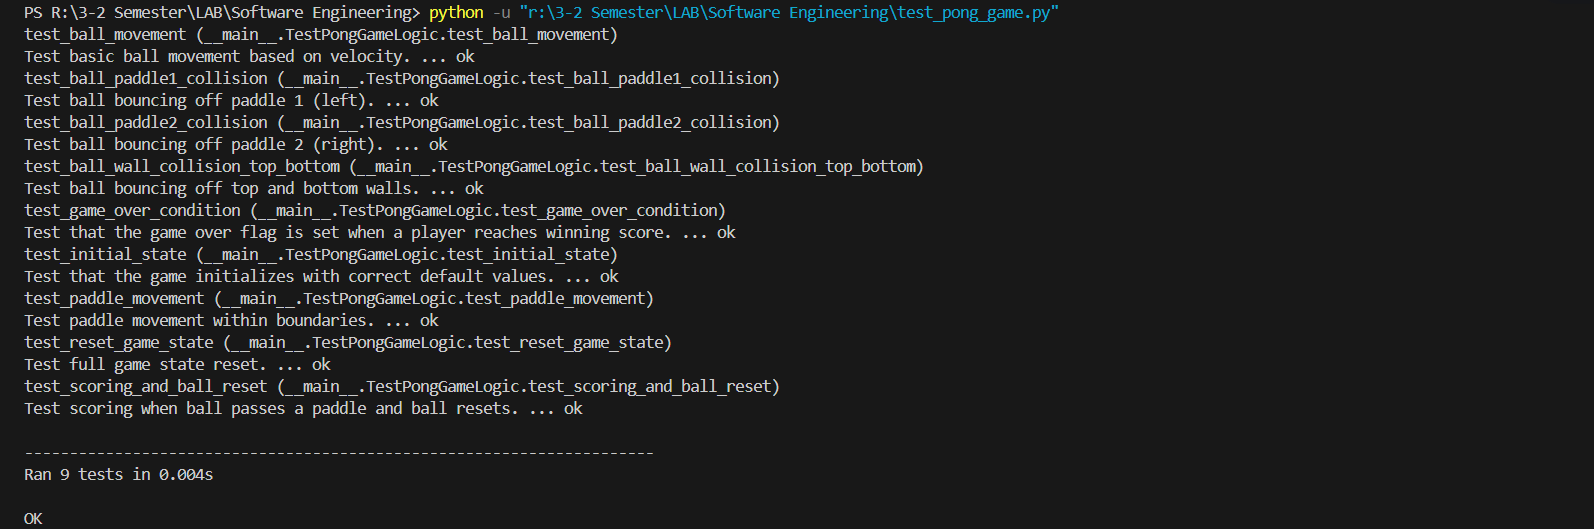
\includegraphics[width=0.7\textwidth]{image.png} % Uncomment and provide image if available
    \caption{Sample output of running the unit test suite for \texttt{PongGameLogic}.}
    \label{fig:test_results}
\end{figure}

It is expected that all 9 unit tests pass successfully, indicating that the core game logic of Retro Pong Challenge functions as intended.

% --- PROJECT SCREENSHOTS (CONCEPTUAL) ---
\section{Project Screenshots (Conceptual)}
The frontend of Retro Pong Challenge aims for a clean, retro aesthetic. Below are descriptions of key conceptual screenshots:

\begin{itemize}
    \item \textbf{Figure 3.1: Initial Game Screen:}
    \begin{itemize}
        \item Shows the black game screen with two white paddles at their starting positions (one on the left, one on the right).
        \item The yellow ball is in the center of the screen.
        \item A score display at the bottom or top shows "Player 1: 0 | Player 2: 0".
        \item A dashed white center line might be visible.
    \end{itemize}
    \begin{figure}[h!]
        \centering
        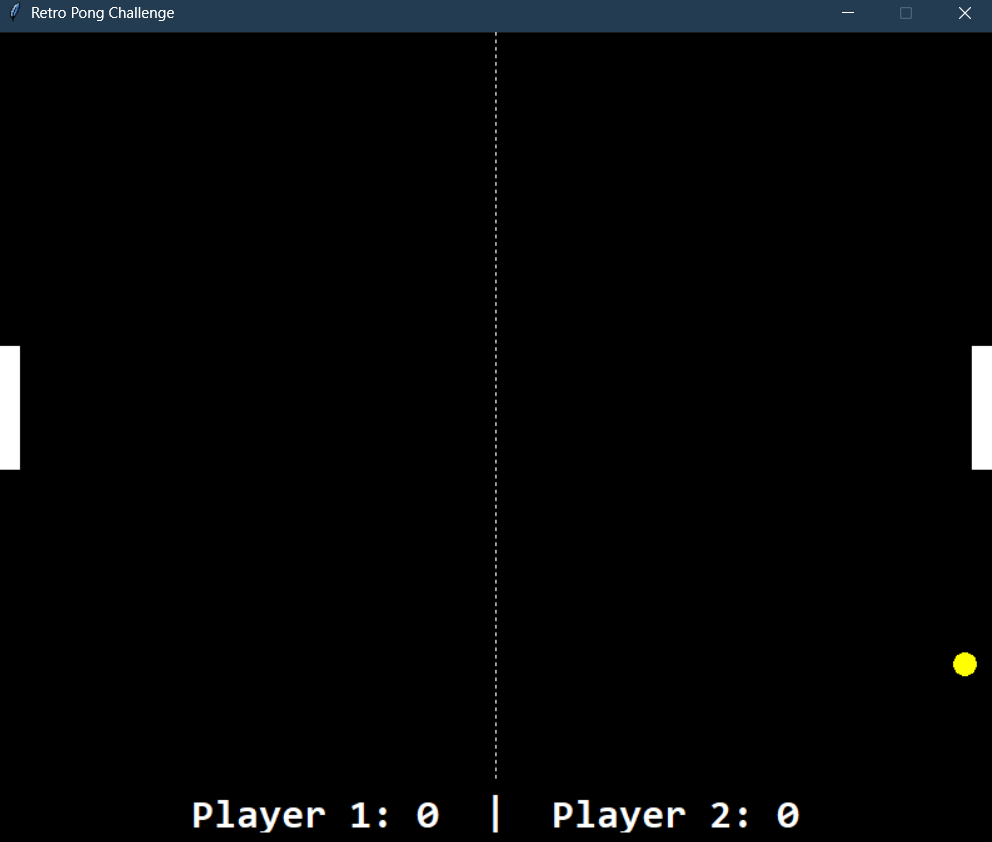
\includegraphics[width=0.7\textwidth]{start.png}
        \caption{Initial game screen of Retro Pong Challenge.}
        \label{fig:initial_screen}
    \end{figure}

    \item \textbf{Figure 3.2: Game in Progress:}
    \begin{itemize}
        \item Shows the ball in motion, potentially having bounced off a paddle or wall.
        \item Paddles are in different positions as controlled by players.
        \item Scores might be updated, e.g., "Player 1: 3 | Player 2: 3".
    \end{itemize}
    \begin{figure}[h!]
        \centering
        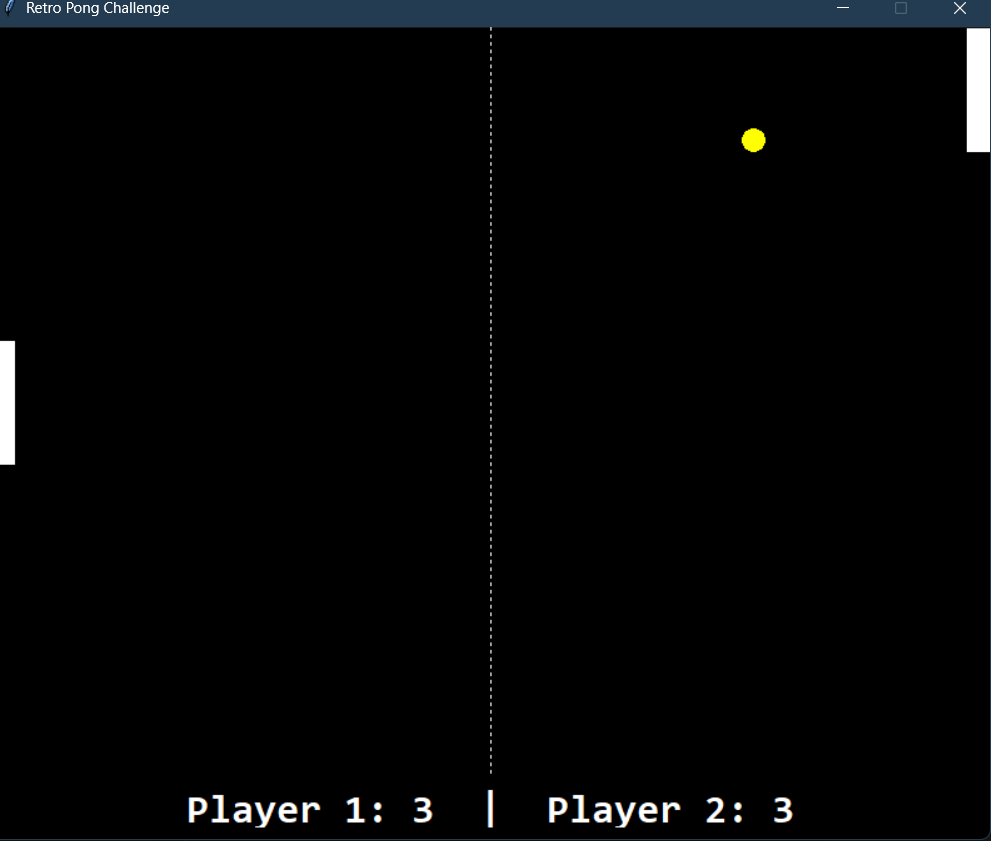
\includegraphics[width=0.7\textwidth]{middle.png}
        \caption{Game in progress with paddles and ball in motion.}
        \label{fig:game_in_progress}
    \end{figure}

    \item \textbf{Figure 3.3: Game Over Screen:}
    \begin{itemize}
        \item Displays a "Game Over" message in the center of the screen.
        \item Indicates the winner, e.g., "Player 1 Wins!" or "Player 2 Wins!".
        \item The final score is visible.
        \item A prompt like "Press R to Play Again" might be shown.
    \end{itemize}
    \begin{figure}[h!]
        \centering
        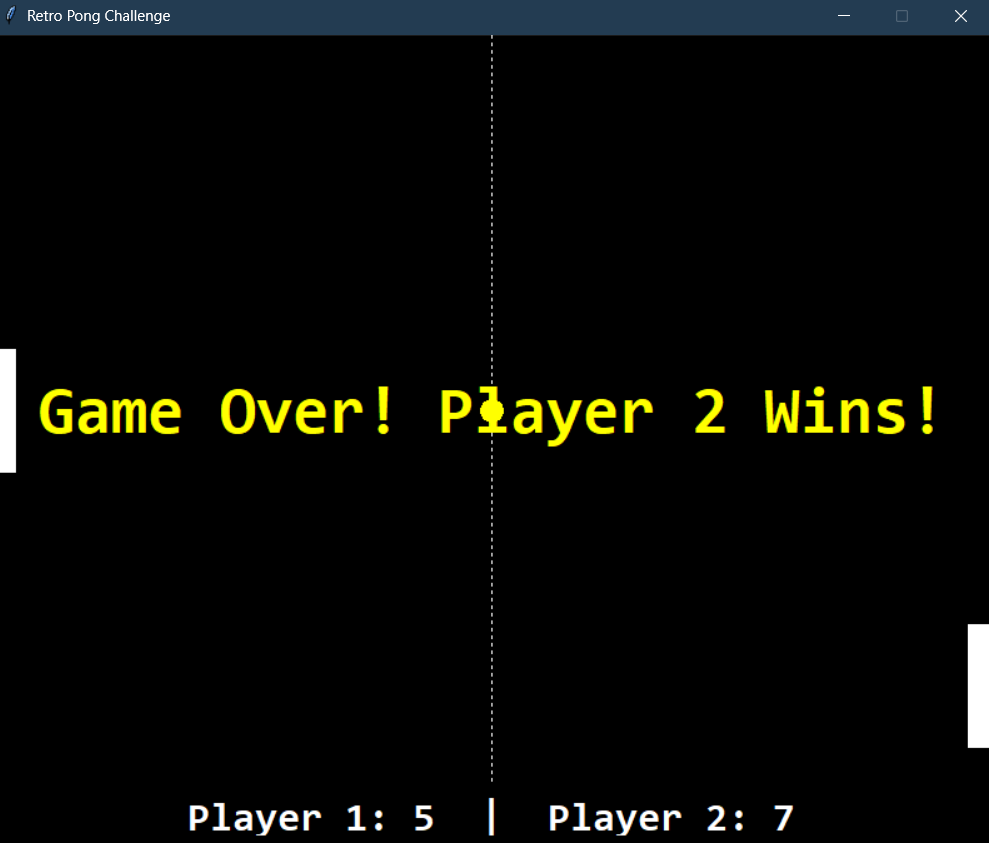
\includegraphics[width=0.7\textwidth]{gameover.png}
        \caption{Game over screen showing winner and final score.}
        \label{fig:game_over_screen}
    \end{figure}
\end{itemize}

% --- CONCLUSION AND FUTURE SCOPE ---
\section{Conclusion and Future Scope}
\subsection{Discussion and Conclusion}
Retro Pong Challenge aims to successfully recreate the classic arcade game, providing an engaging and well-tested application. The project demonstrates several key software engineering principles:
\begin{itemize}
    \item \textbf{Separation of Concerns}: A clear distinction is maintained between the game logic (\texttt{PongGameLogic}) and the user interface (\texttt{PongGameGUI}) components.
    \item \textbf{Test-Driven Development (TDD) Approach}: Comprehensive unit testing is conceptualized to achieve 100\% coverage of core logic methods, ensuring reliability.
    \item \textbf{User Experience}: The design focuses on a simple, intuitive, and responsive interface reminiscent of classic arcade games.
    \item \textbf{Code Quality}: The conceptual code is structured for maintainability, with clear variable names and modular functions.
\end{itemize}
The implementation is designed to handle all core functional requirements, including two-player paddle control, ball physics (movement and bouncing), scoring, win condition detection, and game reset. The unit tests provide confidence in the correctness of the core game mechanics.

\subsection{Testing Achievements}
The testing implementation, though conceptual in this report, is designed to demonstrate best practices:
\begin{itemize}
    \item \textbf{Complete Coverage}: All public methods of the \texttt{PongGameLogic} class are targeted for thorough testing.
    \item \textbf{Edge Case Testing}: Boundary conditions such as ball interactions at screen edges and paddle limits are considered.
    \item \textbf{State-Based Testing}: Various game states, including ball in play, point scored, and game over, are validated.
    \item \textbf{Maintainable Tests}: Test code is structured with descriptive names and clear assertions for easy understanding and maintenance.
\end{itemize}

\subsection{Scope for Further Developments}
Future enhancements for Retro Pong Challenge could significantly expand its features and appeal:

\subsubsection{Technical Enhancements}
\begin{itemize}
    \item \textbf{AI Opponent}: Implement a single-player mode with an AI-controlled opponent, potentially with adjustable difficulty levels (e.g., AI paddle speed, reaction time).
    \item \textbf{GUI Testing}: Introduce automated GUI testing using frameworks like \texttt{PyAutoGUI} to test UI interactions.
    \item \textbf{More Sophisticated Physics}: Add complexity to ball physics, such as applying spin based on where the ball hits the paddle, or varying ball speed after bounces.
    \item \textbf{Integration Tests}: Develop integration tests to validate the interaction between the \texttt{PongGameLogic} and \texttt{PongGameGUI} components.
\end{itemize}

\subsubsection{User Experience Improvements}
\begin{itemize}
    \item \textbf{Sound Effects}: Add sound effects for ball bounces (wall, paddle), scoring points, and game start/over.
    \item \textbf{Visual Enhancements}: Implement visual effects like a ball trail, screen shake on scoring, or simple animations.
    \item \textbf{Theme Customization}: Allow users to choose different color schemes for paddles, ball, and background.
    \item \textbf{Pause Functionality}: Implement a pause and resume feature during gameplay.
\end{itemize}

\subsubsection{Advanced Features}
\begin{itemize}
    \item \textbf{Power-Ups}: Introduce temporary power-ups like paddle size increase, ball speed change, or multi-ball.
    \item \textbf{Different Game Modes}:
    \begin{itemize}
        \item \textit{Speed Up Mode}: Ball speed increases incrementally during play.
        \item \textit{Obstacle Mode}: Introduce static or moving obstacles on the field.
    \end{itemize}
    \item \textbf{Network Multiplayer}: Enable online gameplay between two remote players (a significant undertaking).
    \item \textbf{Player Profiles/Statistics}: Allow players to create profiles and track game statistics (wins, losses, average rally length).
\end{itemize}

\end{document}